\chapter{図表の配置}
\label{ch:figure_table}

\LaTeX で図や表を挿入するときのコマンドは初心者には覚えにくいです.
また,インターネットで検索したものを継ぎ接ぎした結果何が何だかよくわからないコードができあがるということがよく起きるのでこのファイルからコピーアンドペーストすれば問題ないようにしておきました.

\section{図の配置}
\label{sec:figure}

\subsection{図を1枚だけ配置する方法}
\label{ssec:figure_sigle}

ここでは図を1枚だけ配置する方法を紹介します.
図を配置するときは \verb|figure| 環境で図を自動配置し,\verb|\includegraphics| で図を挿入します(図~\ref{fig:one_figure}のコードを参照).
\verb|figure| のオプション \verb|[]| の中にある文字は出力する場所を示します.
\begin{itemize}
    \item \verb|t|\quad ページ上部(\textbf{t}op)に図を出力
    \item \verb|b|\quad ページ下部(\textbf{b}ottom)に図を出力
    \item \verb|p|\quad 単独ページ(\textbf{p}age)に図を出力
    \item \verb|h|\quad できるだけその位置(\textbf{h}ere)に図を出力
    \item \verb|H|\quad 必ずその位置(\textbf{H}ere)に図を出力
\end{itemize}
学位論文中の図は原則ページ上部に配置するのでこの \verb|tex| ファイル中では \verb|[tp]| に設定してあります.
皆さんはこのままコピーしてください.
\verb|\columnwidth| は現在のコラムのテキスト幅を指しており,\verb|[width=0.5\columnwidth]| と設定することで,テキスト幅の半分の横幅で図を挿入できます.

\begin{figure}[tp]
    \centering
    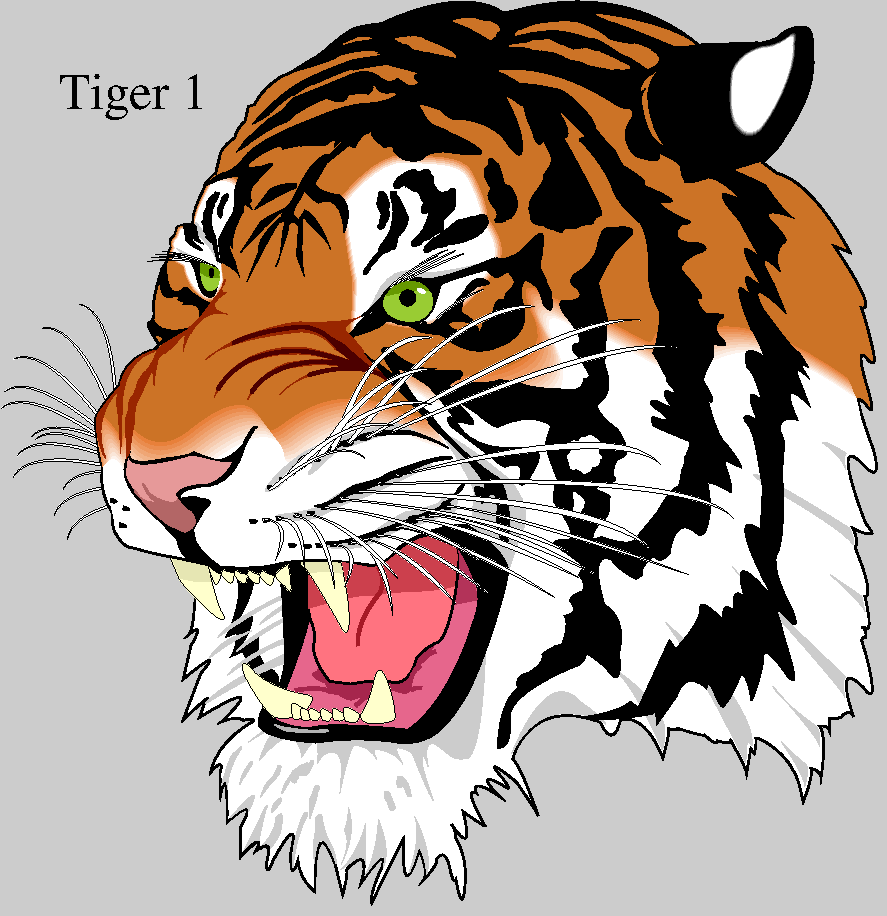
\includegraphics[width=0.5\columnwidth]{figure/tiger1.pdf}
    \caption{1 枚の図.}
    \label{fig:one_figure}
\end{figure}


\subsection{図を複数枚配置する方法}
\label{ssec:multiple}

関連する図を複数枚配置するときは \verb|subfigure| 環境を使いましょう.
例えば 2 枚の図を横に並べて配置したいときは図~\ref{fig:two_figures}のようになります.
ここでは \verb|\hfill| を使って図と図の間の空白を設定していますが,\verb|\hspace{3mm}| のように設定しても構いません.
\verb|\hspace{3mm}| の場合,水平方向に$\SI{3}{\milli\meter}$の空白ができます.
3 枚の図を横に並べたいときも同様で,図~\ref{fig:three_figures}のようになります.
関連する図を横だけでなく縦方向にも配置したいときは,図~\ref{fig:four_figures}のように横並びの \verb|\columnwidth| の合計が大きくなりすぎると自動的に縦に配列してくれます.
ここでは縦方向のスペースを確保するために \verb|\vspace{5mm}| を挿入しています.
また,\verb|subfigure| 環境を使うことでそれぞれの図にラベルを付けることができます.


\begin{figure}[tp]
    \centering
    \begin{subfigure}{0.45\columnwidth}
        \centering
        \includegraphics[width=\columnwidth]{example-image-a}
        \caption{左の図.}
        \label{fig:two_figures_a}
    \end{subfigure}
    \hfill % ここで空白を入れると図が適切に配置される
    \begin{subfigure}{0.45\columnwidth}
        \centering
        \includegraphics[width=\columnwidth]{example-image-b}
        \caption{右の図.}
        \label{fig:two_figures_b}
    \end{subfigure}
    \caption{左右の図.}
    \label{fig:two_figures}
\end{figure}

\begin{figure}[tp]
    \centering
    \begin{subfigure}{0.32\columnwidth}
        \centering
        \includegraphics[width=\columnwidth]{example-image-a}
        \caption{左の図.}
        \label{fig:three_figures_a}
    \end{subfigure}
    \hfill % ここで空白を入れると図が適切に配置される
    \begin{subfigure}{0.32\columnwidth}
        \centering
        \includegraphics[width=\columnwidth]{example-image-b}
        \caption{中央の図.}
        \label{fig:three_figures_b}
    \end{subfigure}
    \hfill % ここで空白を入れると図が適切に配置される
    \begin{subfigure}{0.32\columnwidth}
        \centering
        \includegraphics[width=\columnwidth]{example-image-c}
        \caption{右の図.}
        \label{fig:three_figures_c}
    \end{subfigure}
    \caption{3 枚の図.}
    \label{fig:three_figures}
\end{figure}

\begin{figure}[tp]
    \centering
    % 上の行
    \begin{subfigure}{0.45\columnwidth}
        \centering
        \includegraphics[width=\columnwidth]{example-image-a}
        \caption{左上の図}
        \label{fig:sub1}
    \end{subfigure}
    \hfill % 水平方向のスペース
    \begin{subfigure}{0.45\columnwidth}
        \centering
        \includegraphics[width=\columnwidth]{example-image-b}
        \caption{右上の図}
        \label{fig:sub2}
    \end{subfigure}

    \vspace{5mm} % 縦方向のスペース
    % 下の行
    \begin{subfigure}{0.45\columnwidth}
        \centering
        \includegraphics[width=\columnwidth]{example-image-c}
        \caption{左下の図}
        \label{fig:sub3}
    \end{subfigure}
    \hfill % 水平方向のスペース
    \begin{subfigure}{0.45\columnwidth}
        \centering
        \includegraphics[width=\columnwidth]{example-image-c}
        \caption{右下の図}
        \label{fig:sub4}
    \end{subfigure}
    \caption{上下左右に4つ配置された図}
    \label{fig:four_figures}
\end{figure}




\subsection{画像のファイル形式}
\label{ssec:figure_format}



\section{表の配置}
\label{sec:table}






